\section{The ortholog conjecture in the context of evolutionary theory}

Much of the theory that forms the historical basis of the ortholog conjecture in grounded in proposed scenarios about the evolutionary fate of duplicate genes; giving a narrow focus within this subfield to the theories of sub-functionalization and neo-functionalization.  While gene duplication is certainly important; and it is highly likely that the two aforementioned theories play an important role when duplicate genes are retained, they only represent two scenarios that could befall duplicate genes.

Not only does much of the historical basis behind the OC narrowly focus its attentions on two theories regarding the fate of duplicate genes it also lack a broader biological perspective; failing to take into account important forces that play a role in creating \textcolor{red}{phenotypic and genetic} distinctions between different species.

The development of hybrid incompatibilities is an important step in distinct organism arising from a population that was previously considered a single species.  \textcolor{red}{One of the more plausible} theories explaining the manner in which genetic incompatibilities arise is Dobzhansky-Muller model.  The Dobzhansky-Muller model of hybrid incompatibilities attempts to explain how a particular allele or mutation can cause genetic incompatibilities between organisms while not leading to a decrease in fitness when arising in the genetic background of the original population.  For example, if orga \textcolor{red}{explain the theory here}  

%%%%%%%%%%%%%%%%%%%%%%%%
%%%%%%%%%%%%%%%%%%%%%%%%
%%%%%%%%%%%%%%%%%%%%%%%
%%%%%%%%%%%%%%%%%%%%%%%
\begin{figure}[h!]
\begin{centering}
	\begin{subfigure}[b]{0.45\textwidth}	
		\centering
		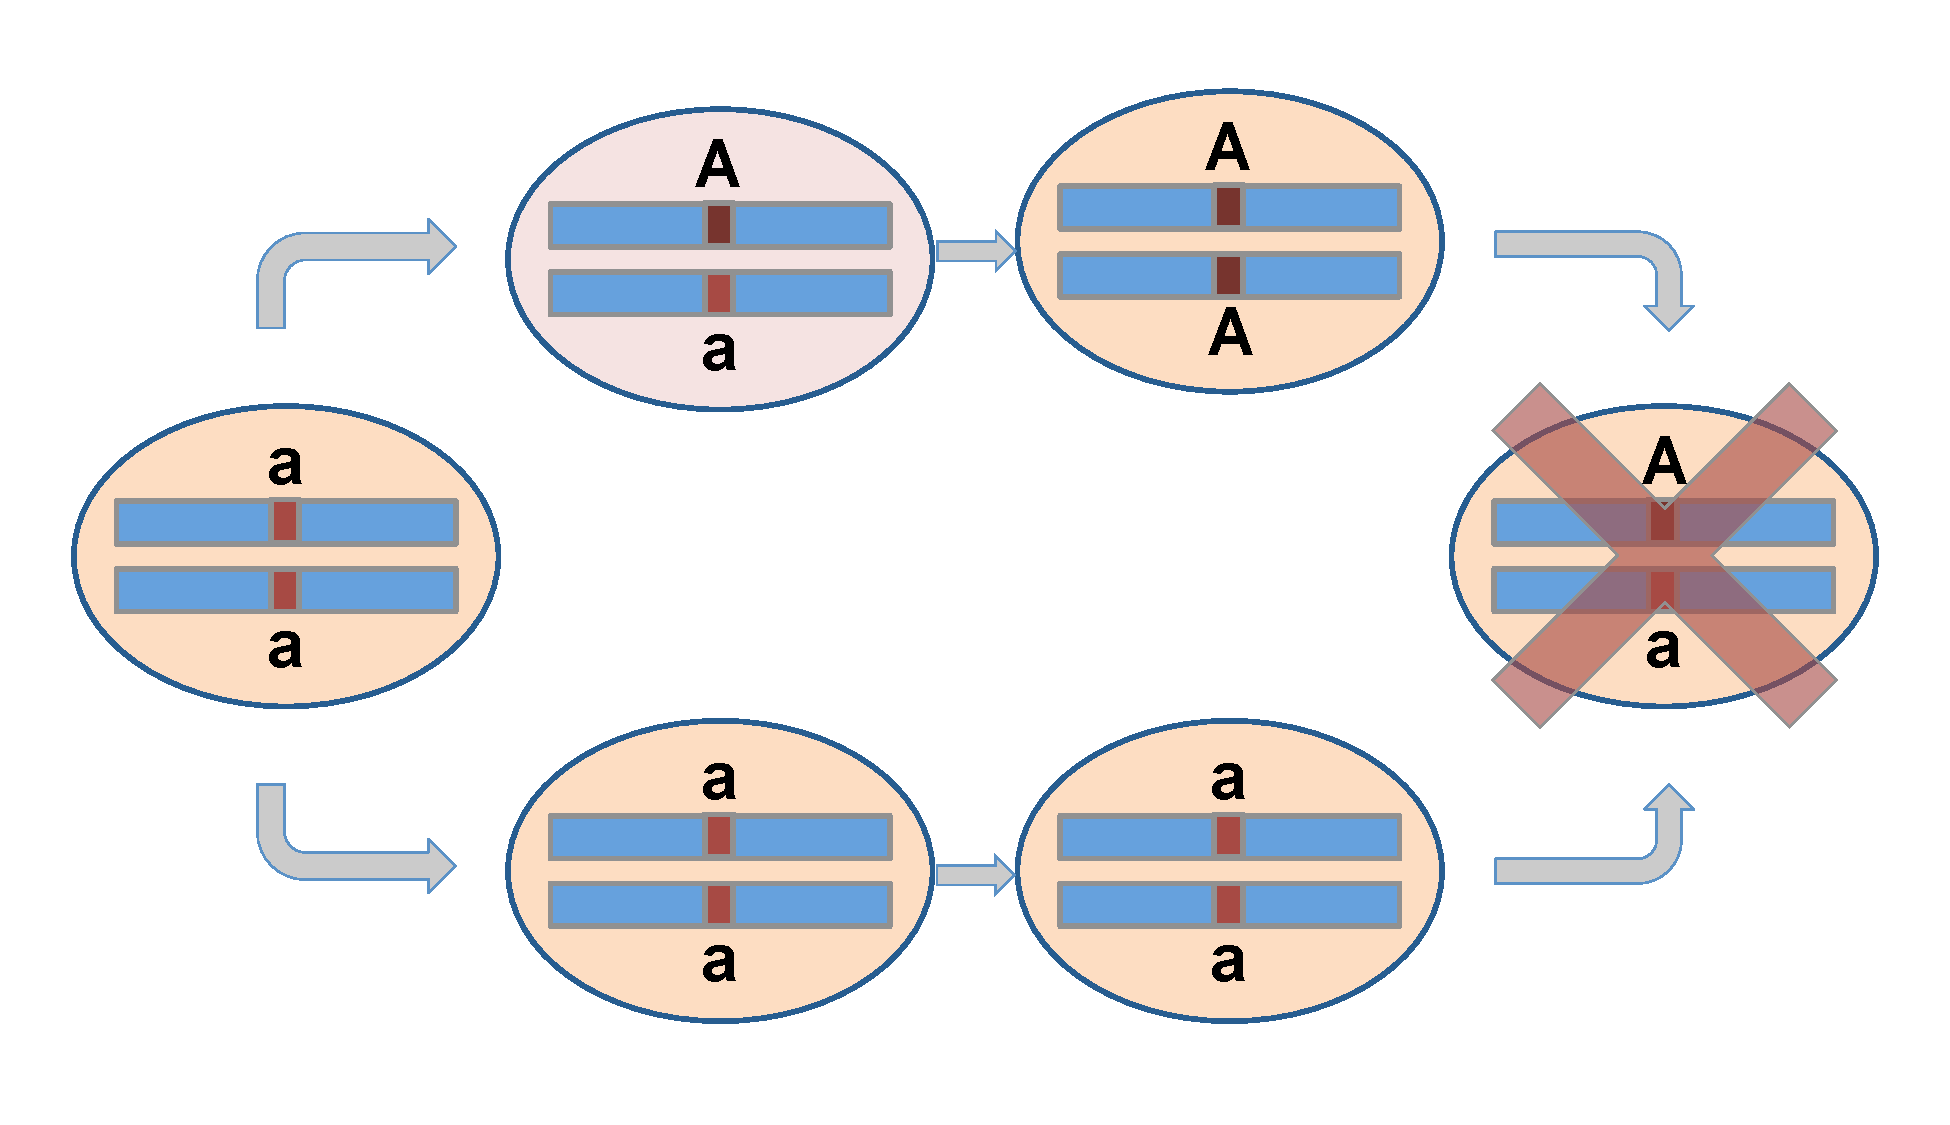
\includegraphics[width=\textwidth]{Figures/dm/DM_1}
		\label{fig:dm1}
		\caption{Single locus model of hybrid incompatibility}
	\end{subfigure}
	\quad
	\begin{subfigure}[b]{0.45\textwidth}	
		\centering
		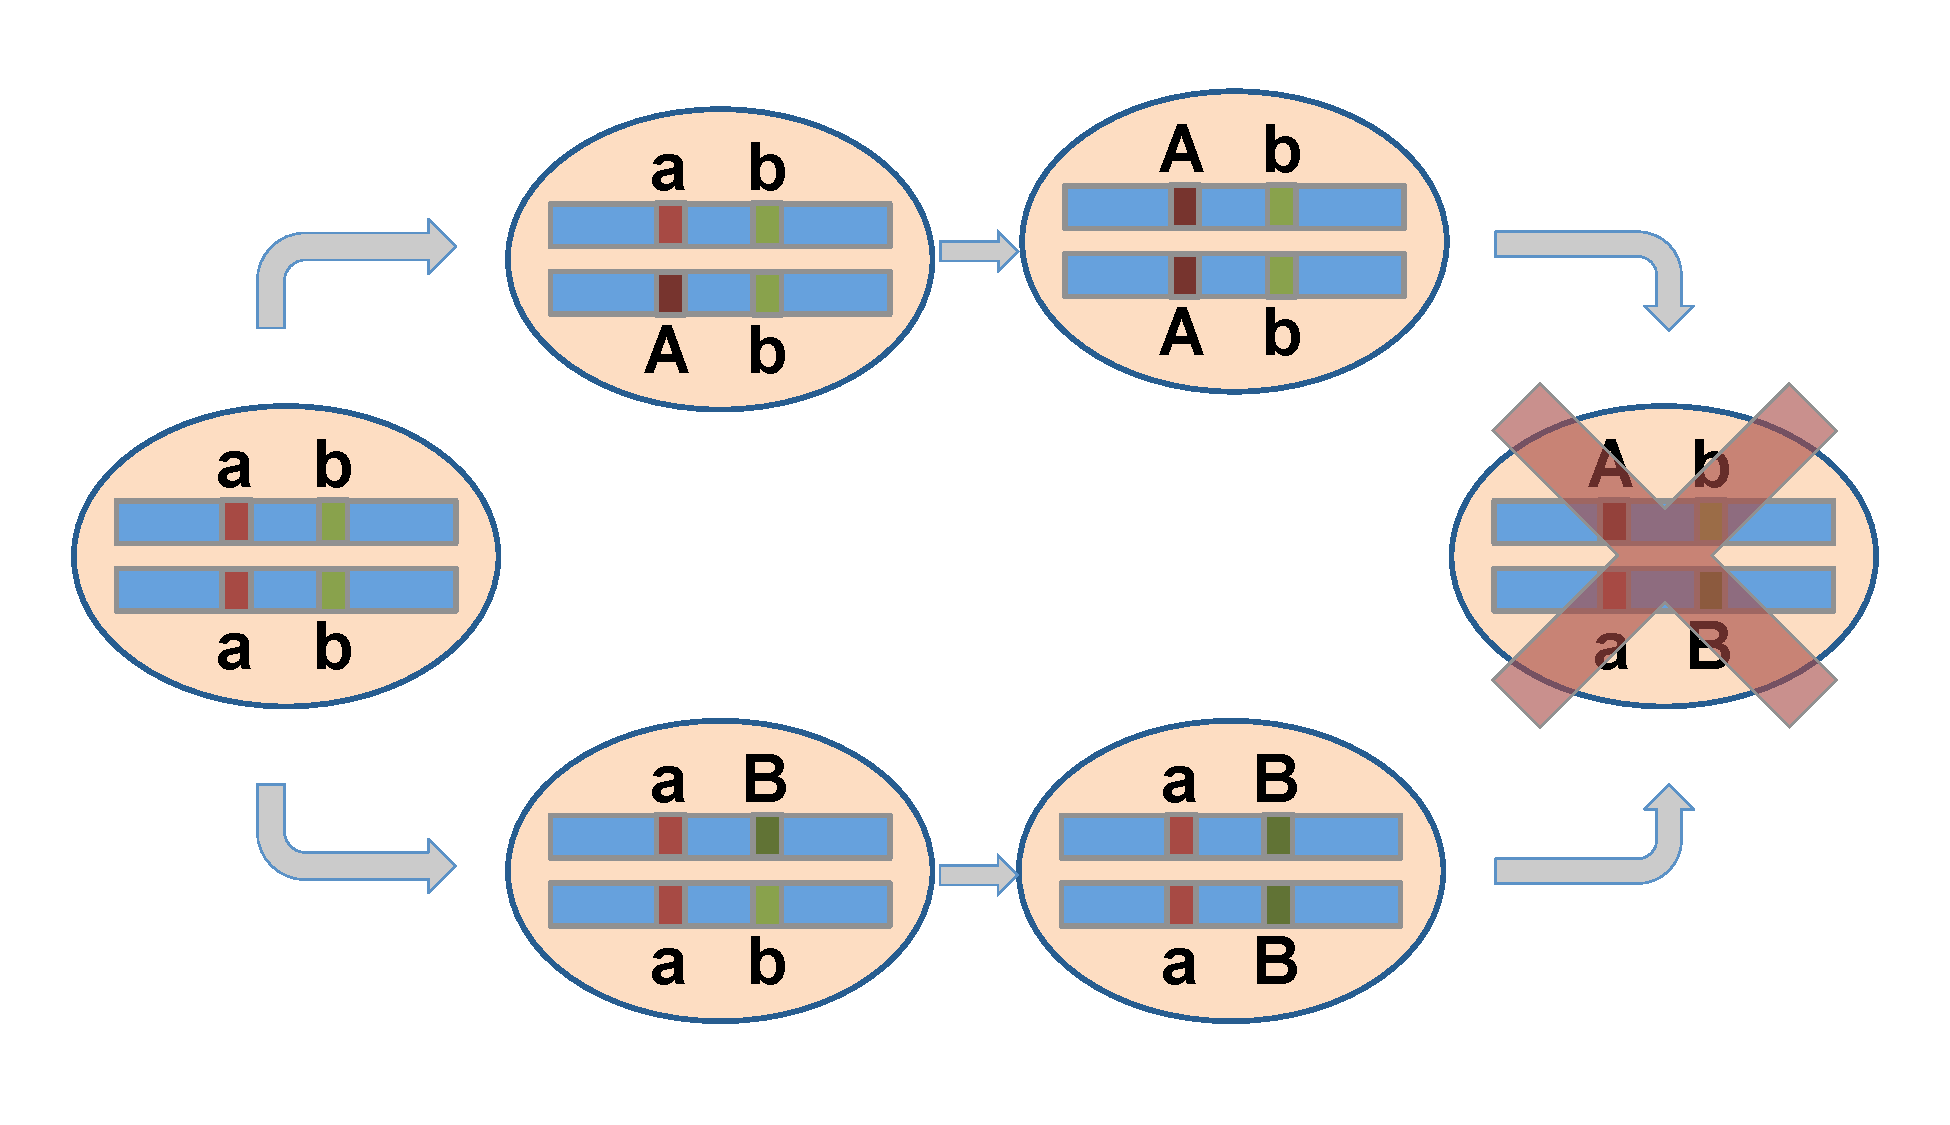
\includegraphics[width=\textwidth]{Figures/dm/DM_2}
		\label{fig:dm2}
		\caption{Two locus model of hybrid incompatibility}
	\end{subfigure}
\end{centering}
	
\caption[Description of the Dobzhansky-Muller model of hybrid incompatibilities]{A figure illustrating the concept behind the Dobzhansky-Muller model of hybrid incompatibilities.  \Cref{fig:dm1} illustrates a single locus model for hybrid incompatibility.  In this model only allele $a$ appears in the ancestral population. After becoming reproductively isolated the $A$ allele appears in one of the pure breeding populations and becomes fixed, but does not appear in the other.  Upon hybridization incompatibility is observed due to the $Aa$ combination of alleles, although this combination was previously experienced (light red organism) but did not result in incompatibilities. \Cref{fig:dm2} illustrates a multi-locus model for the development of hybrid incompatibilities.  In this model incompatibilities can be caused by incompatibilities between the $A$ and $B$ alleles, or by the $Aa$ combination of alleles occurring on the genetic background provided by the $B$ allele. Because the $A$ and $B$ only occurred on the same genetic background the two locus model avoids the problem of explaining how in the single locus model a genetic incompatibility can arise in an ancestral population without that population experiencing the same decrease in fitness as the hybrid species.}

\label{fig:dbm_simple}
\end{figure}
%%%%%%%%%%%%%%%%%%%%%%%
%%%%%%%%%%%%%%%%%%%%%%%

%%%%%%%%%%%%%%%%%%%%%%%%
%%%%%%%%%%%%%%%%%%%%%%%%

The reason for this is that allele A was selected for in the different genetic background that exists in Species 1.  When placed in Species 2 it causes a decrease in fitness because it is operating in a different genetic background.  This can be taken a step further by postulating that this decrease in fitness must be due allele A doing something different: if it was merely inert
Unless one wishes to introduce mysterious chromosomal aberrations to account for the 

The Dobzhansky-Muller model of hybrid incompatibilities provides a strong theoretic argument against the ortholog conjecture; 



%In the absence of a \textcolor{red}{non genetic, whats the term} barrier to reproductive isolation hybrid incompatibilities, either pre or post-zygotic would be the only remaining barrier to 


Mention how duplicated are very unlikely to contribute to chromosomal incompatibilities initially as Lynch states.

Mention Dosage as a potentially more common fate of duplicates.

While duplicate gene subfunctionalization and neo-functionalization have been frequently cited as the theoretic basis for the ortholog conjecture these two theoretic scenarios represent only two of the potential fates of duplicate genes.  Furthermore, 